% Example LaTeX file showing how to include the generated set operation diagrams
% Include this file in your main document or use it as reference

\section{Set Operations with Matplotlib-Generated Diagrams}

\subsection{Combined View (Currently Used in Document)}

% This is the version currently used in chapter_probability.tex
\begin{figure}[h]
    \centering
    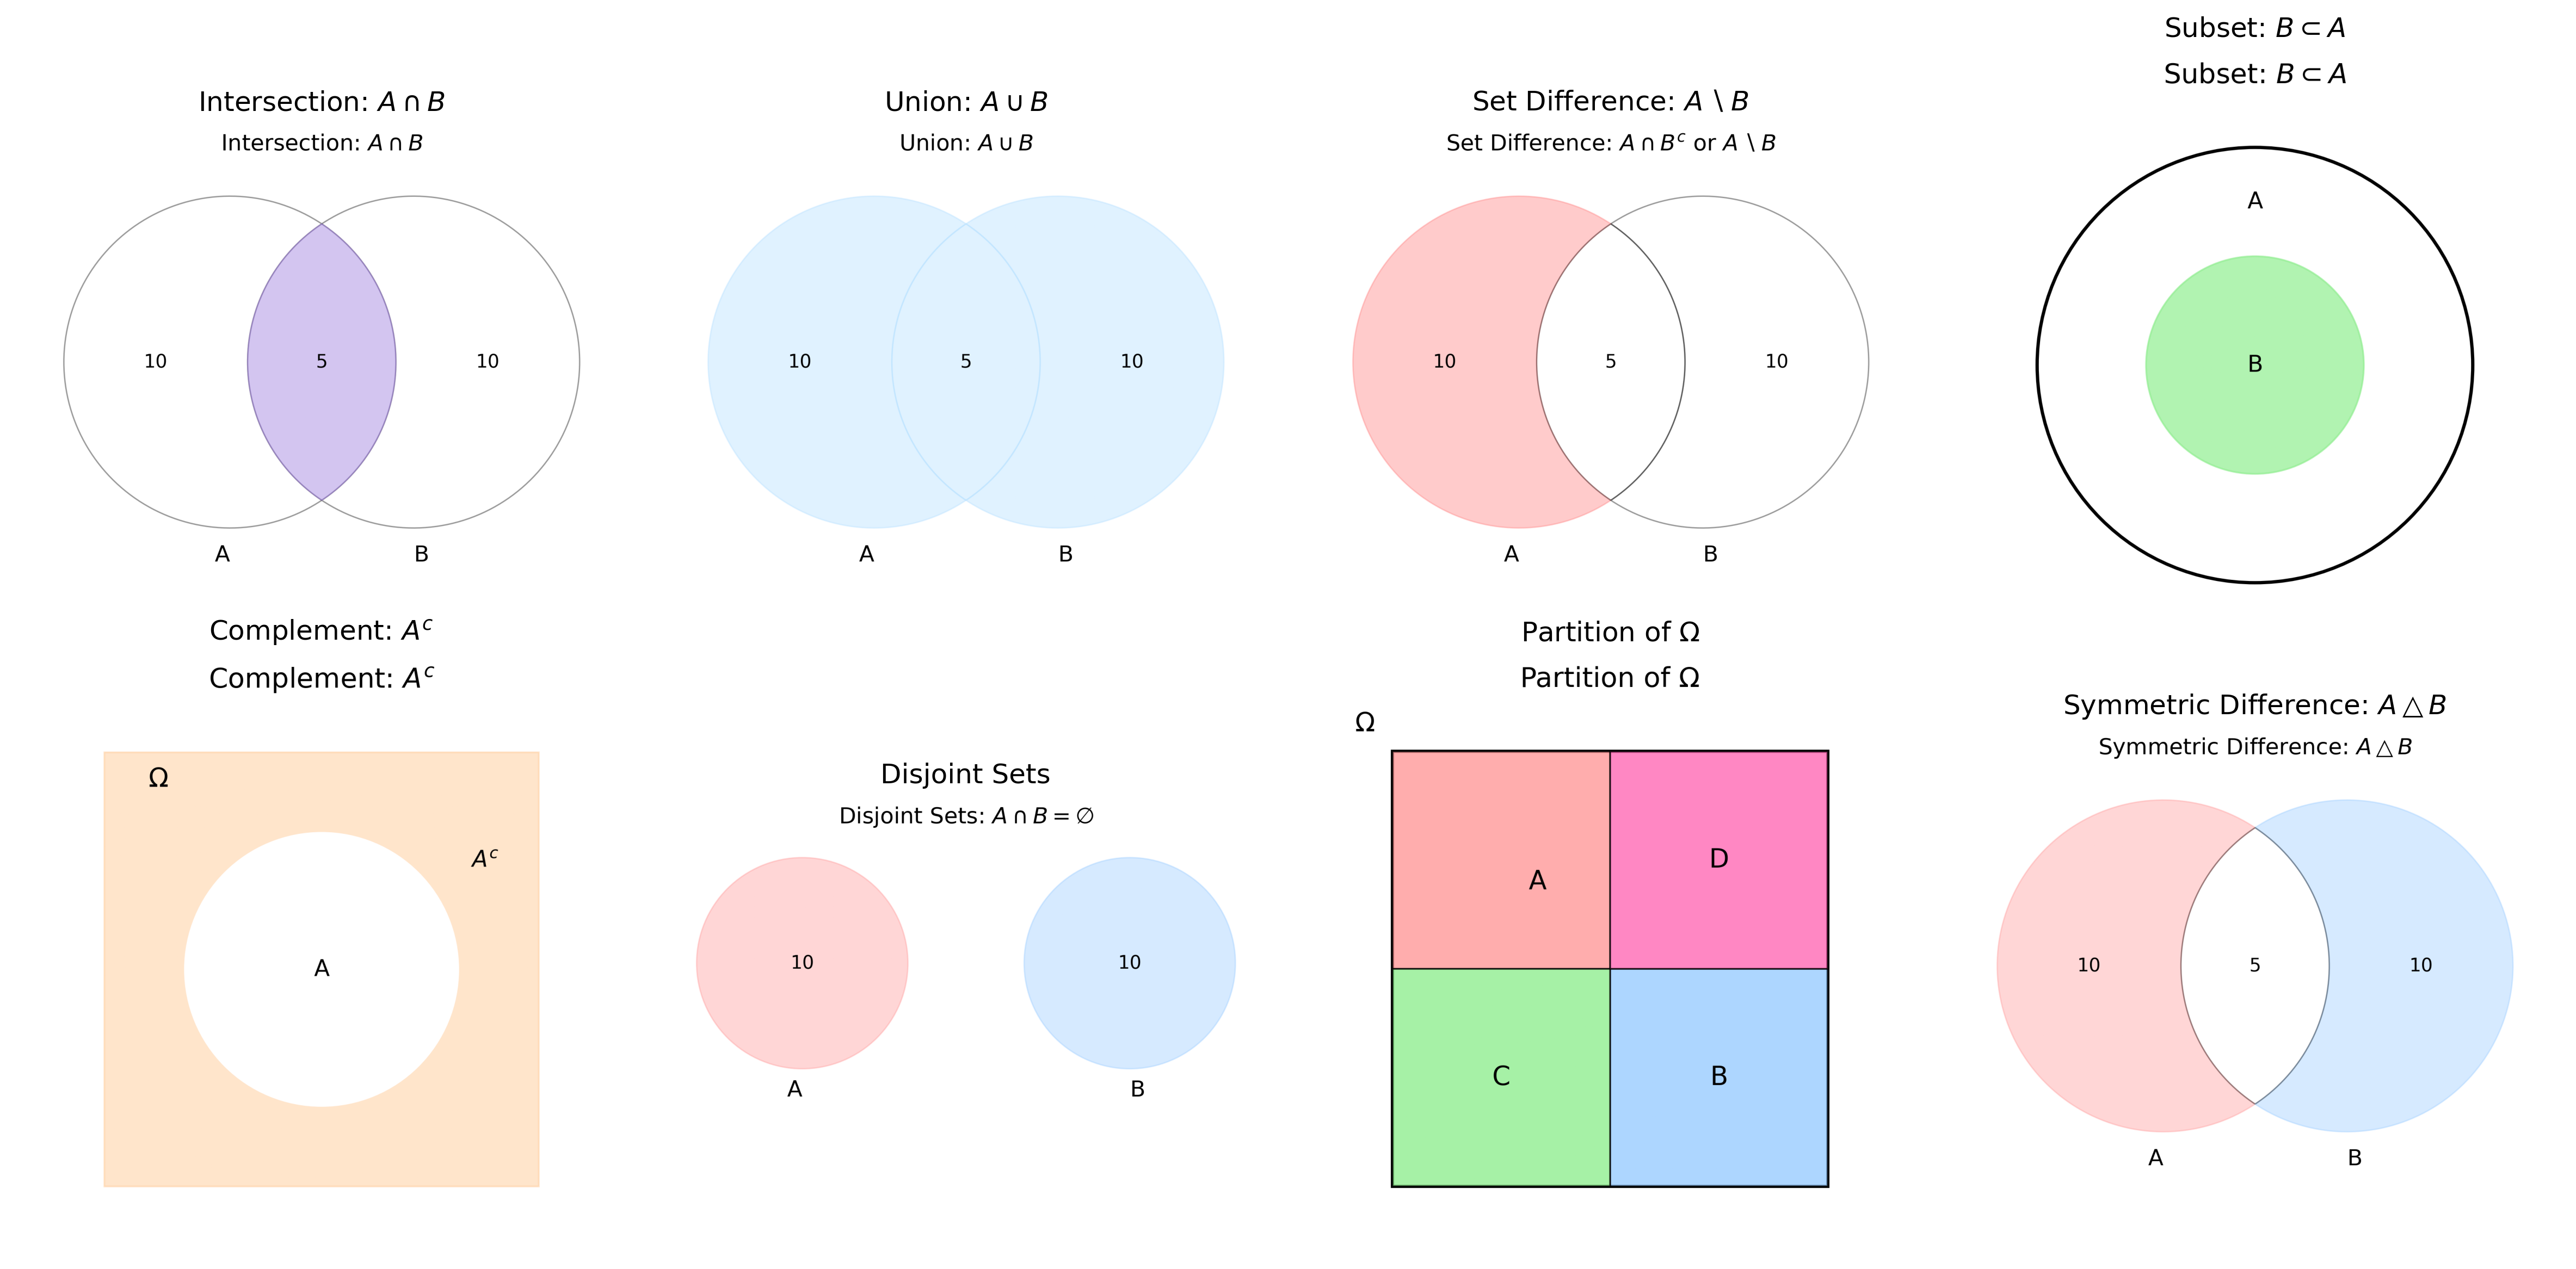
\includegraphics[width=\textwidth]{figures/set_operations/all_operations.png}
    \caption{Visualizations of fundamental set operations}
    \label{fig:set_operations}
\end{figure}

\subsection{Individual Set Operations (Alternative Approach)}

\begin{figure}[h]
    \centering
    \begin{subfigure}{0.48\textwidth}
        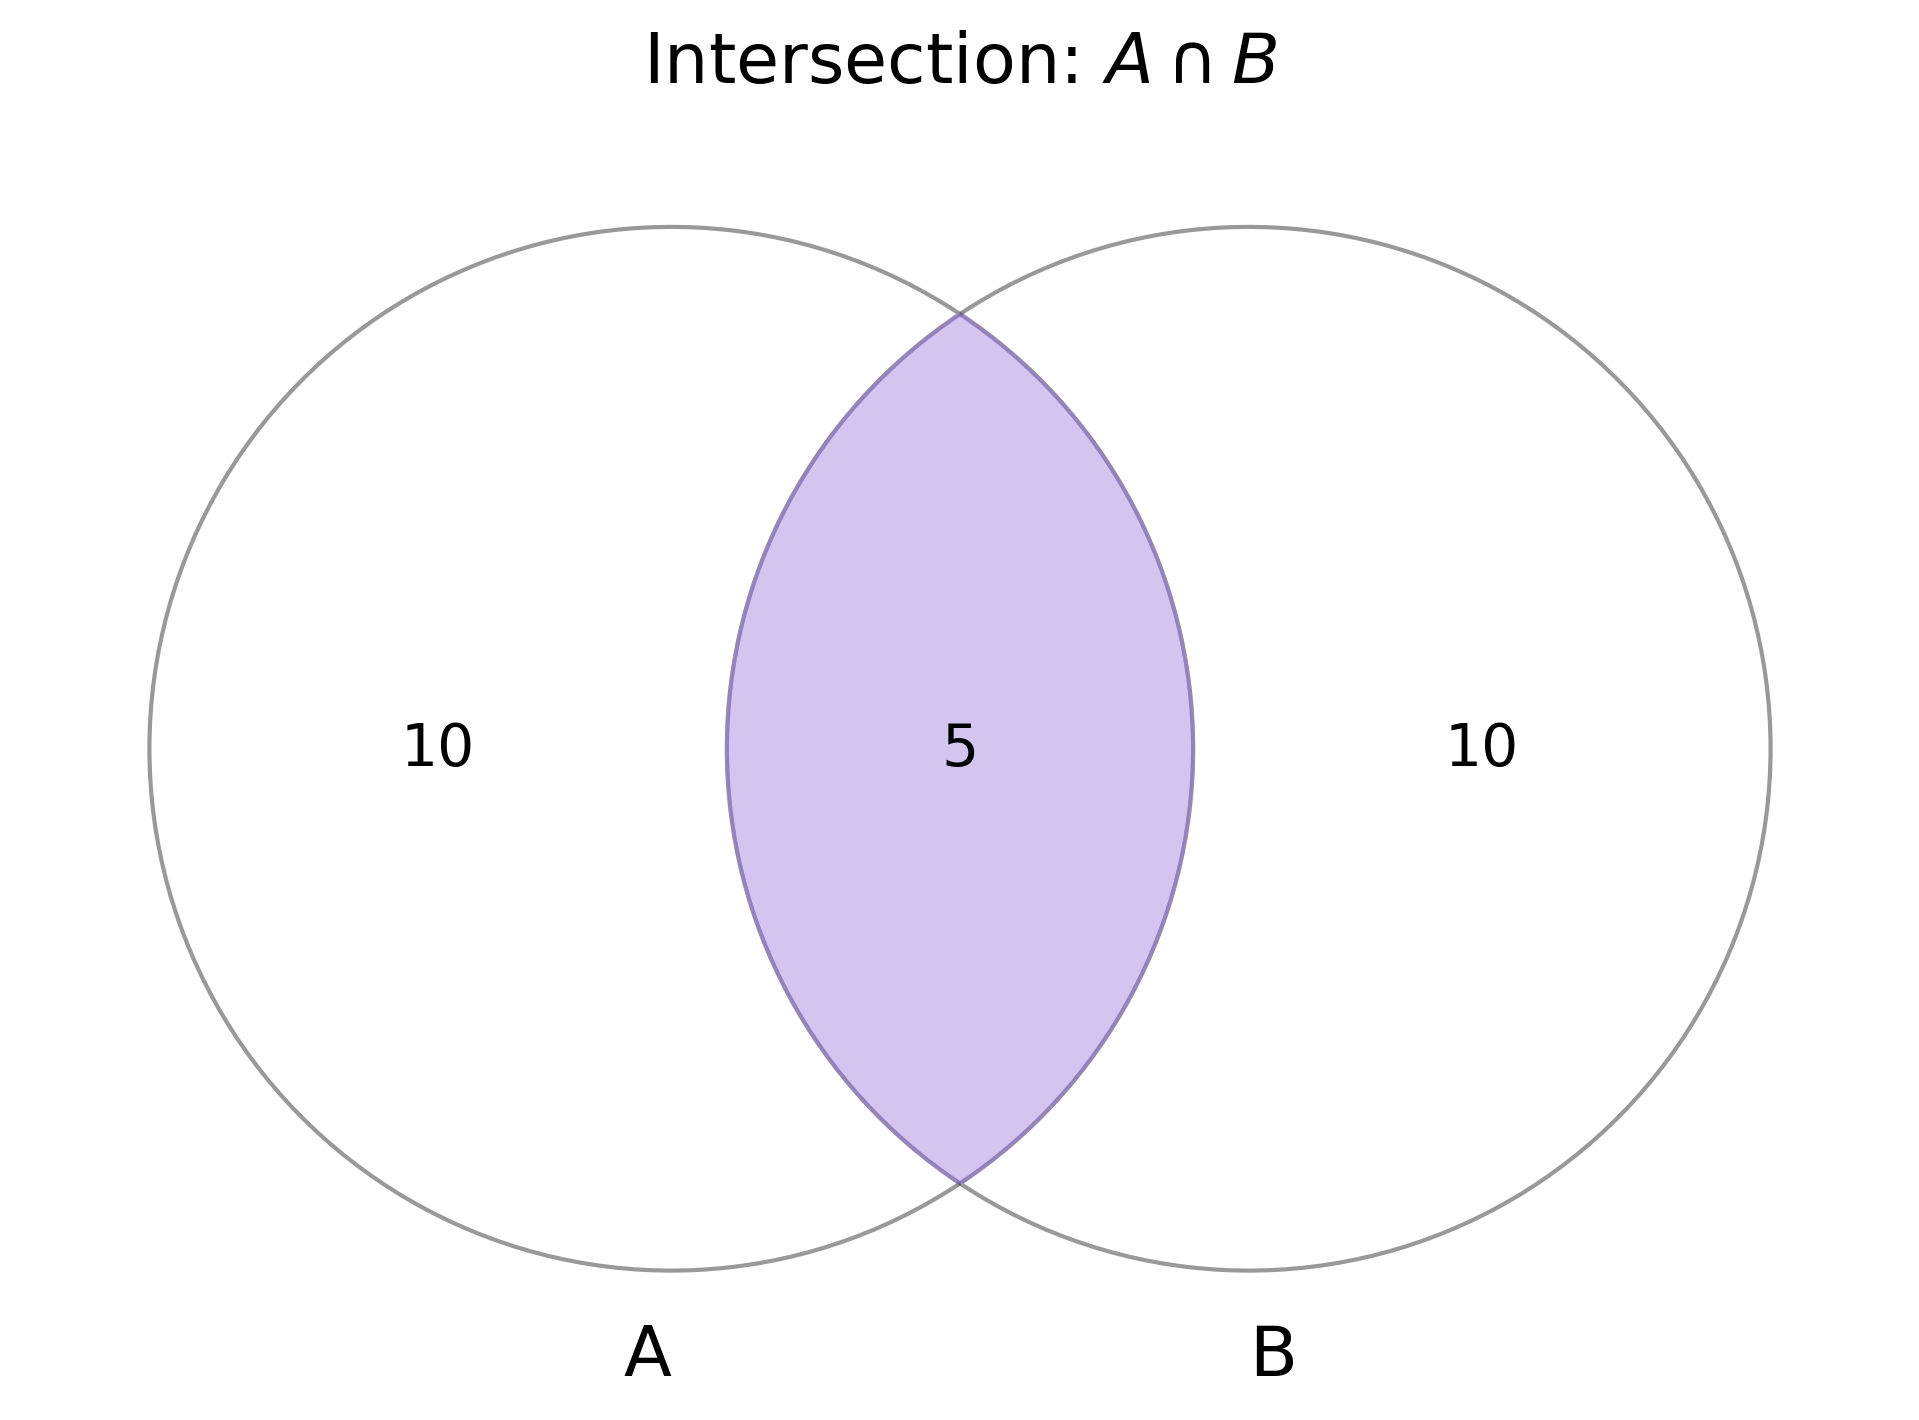
\includegraphics[width=\textwidth]{figures/set_operations/intersection.png}
        \caption{Intersection: $A \cap B$}
        \label{fig:intersection}
    \end{subfigure}
    \hfill
    \begin{subfigure}{0.48\textwidth}
        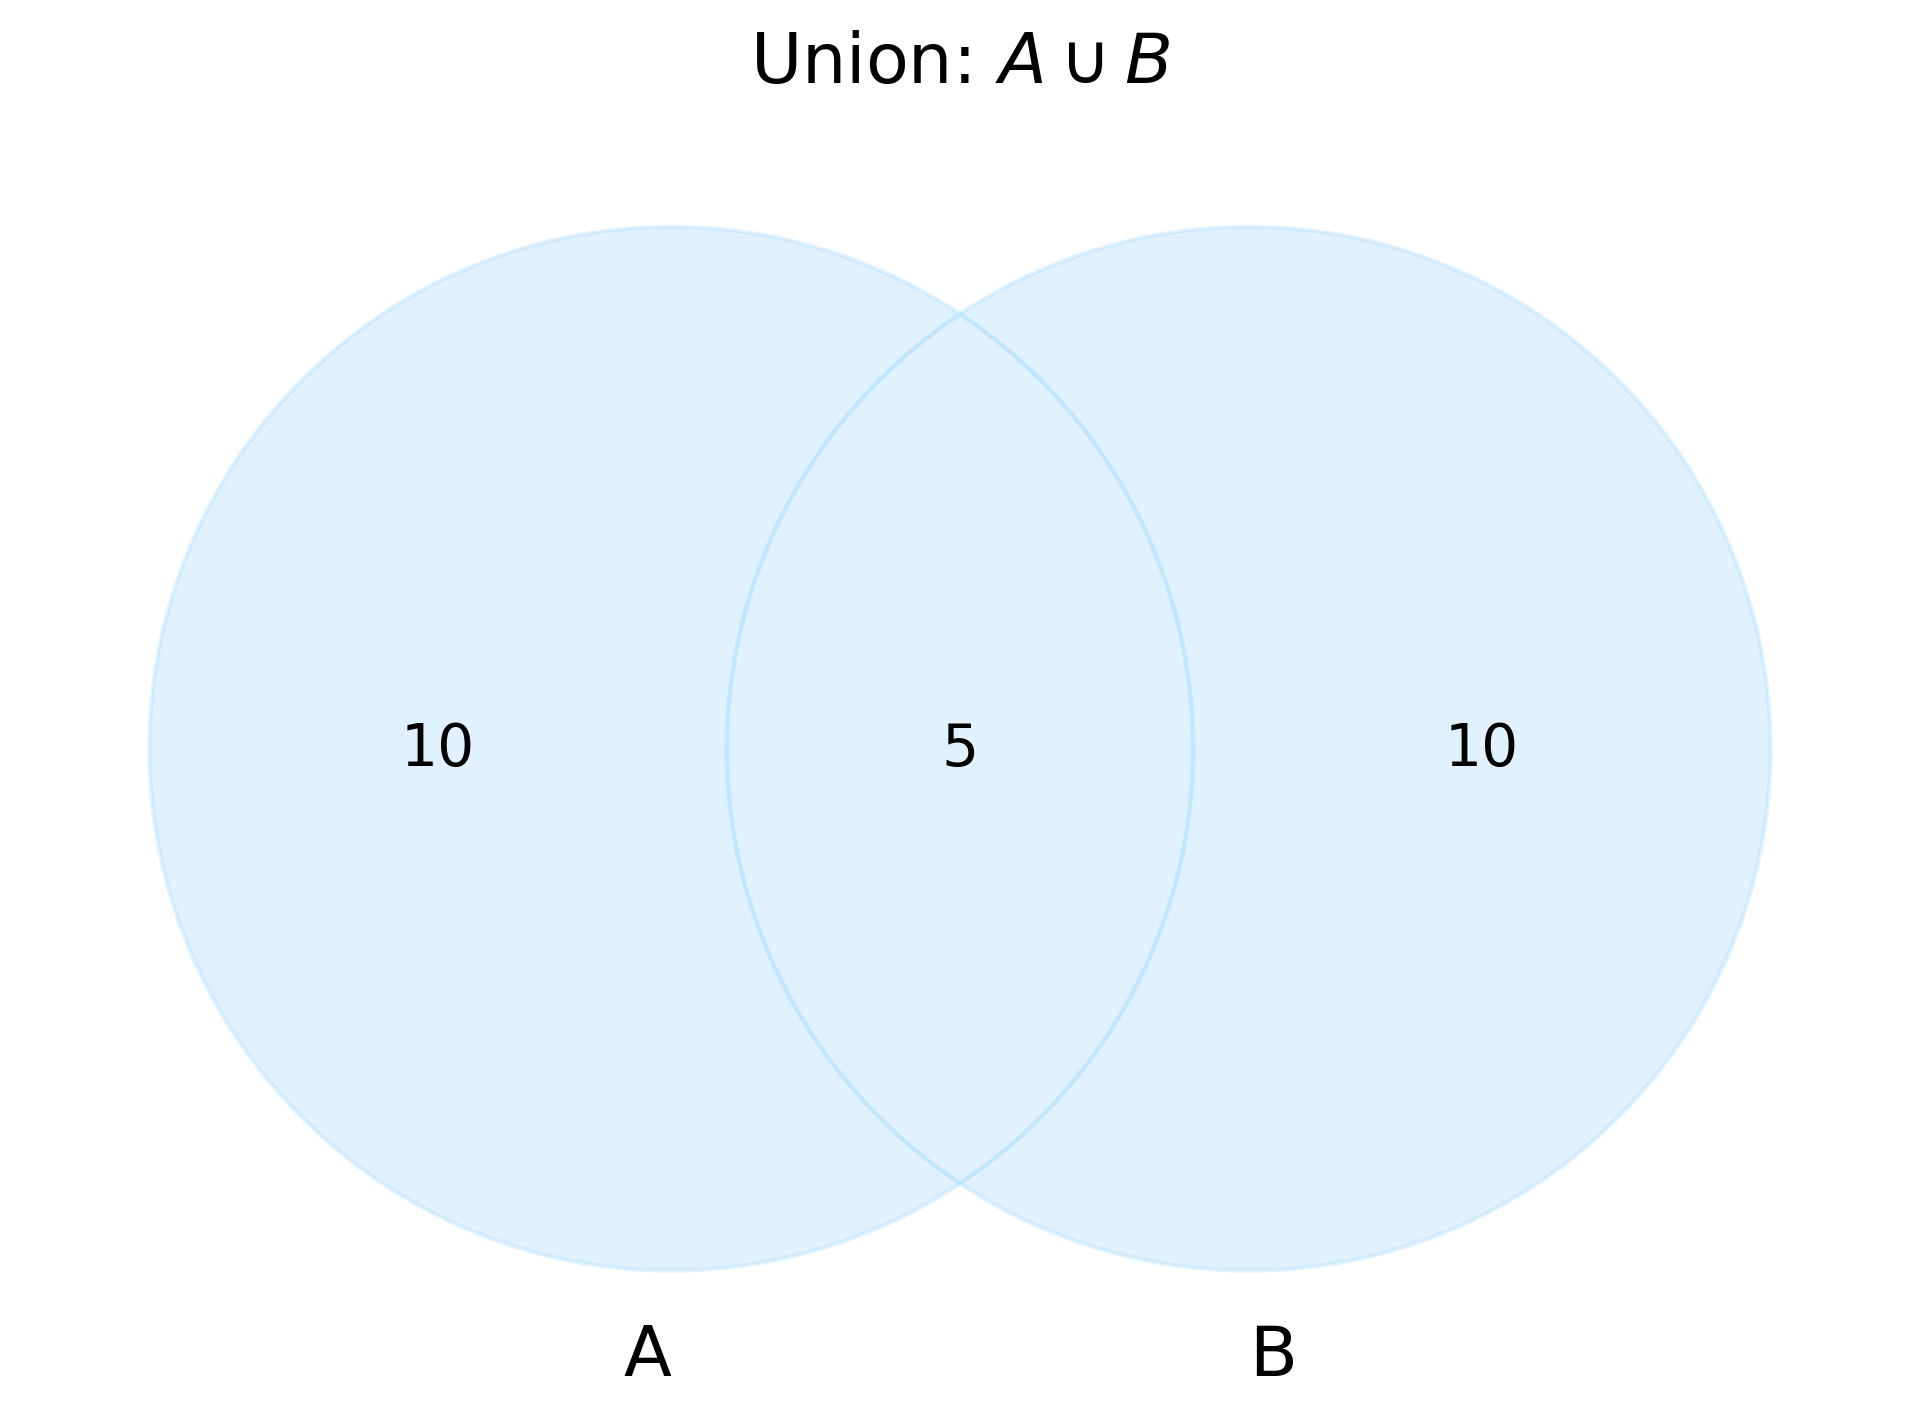
\includegraphics[width=\textwidth]{figures/set_operations/union.png}
        \caption{Union: $A \cup B$}
        \label{fig:union}
    \end{subfigure}
    
    \vspace{0.5cm}
    
    \begin{subfigure}{0.48\textwidth}
        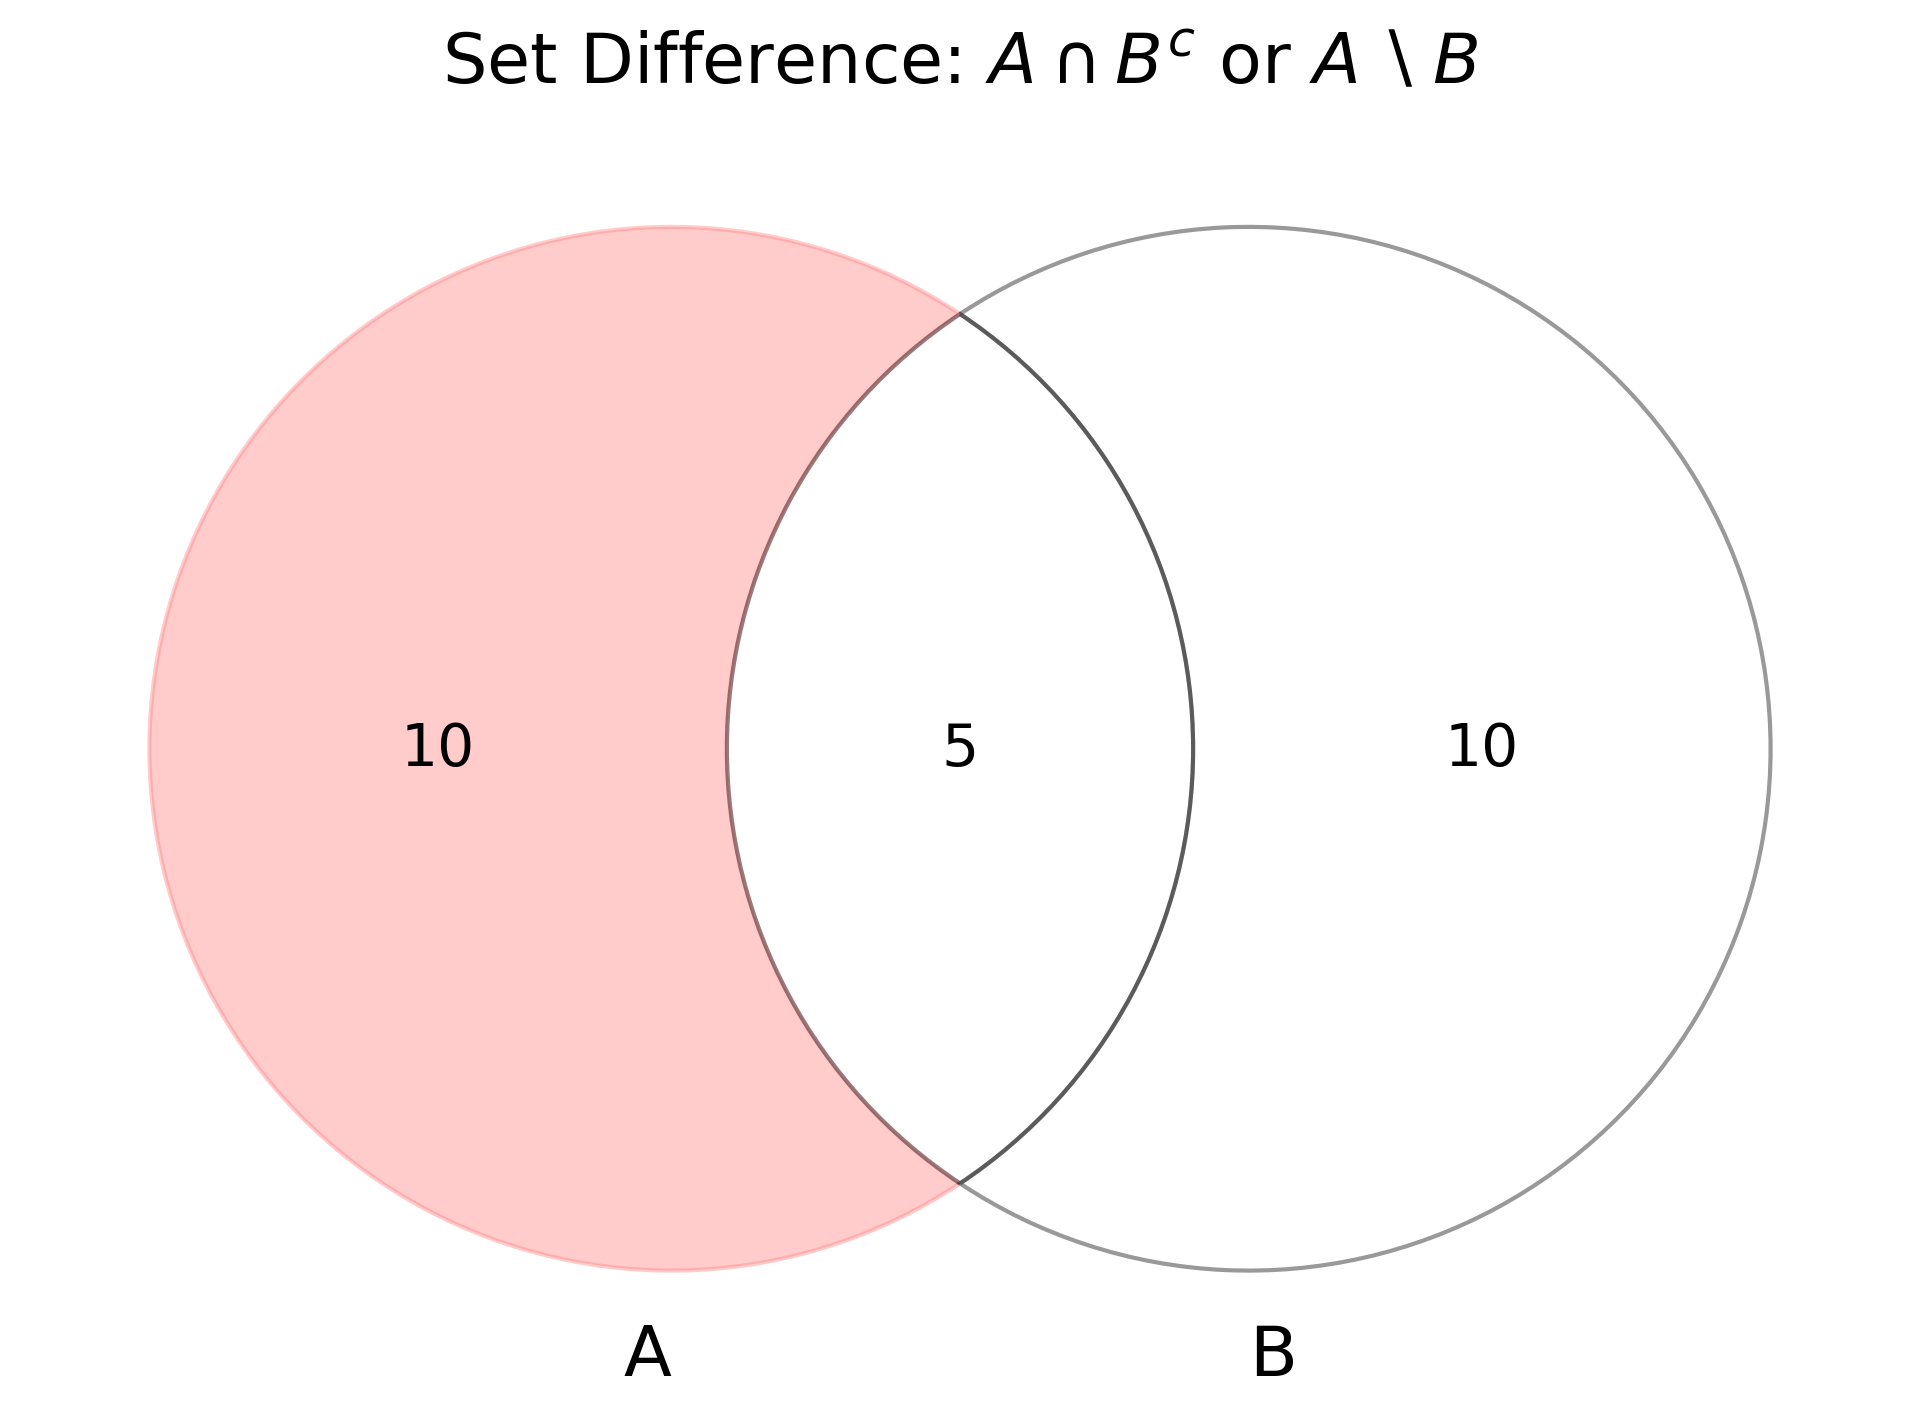
\includegraphics[width=\textwidth]{figures/set_operations/difference.png}
        \caption{Set Difference: $A \setminus B$}
        \label{fig:difference}
    \end{subfigure}
    \hfill
    \begin{subfigure}{0.48\textwidth}
        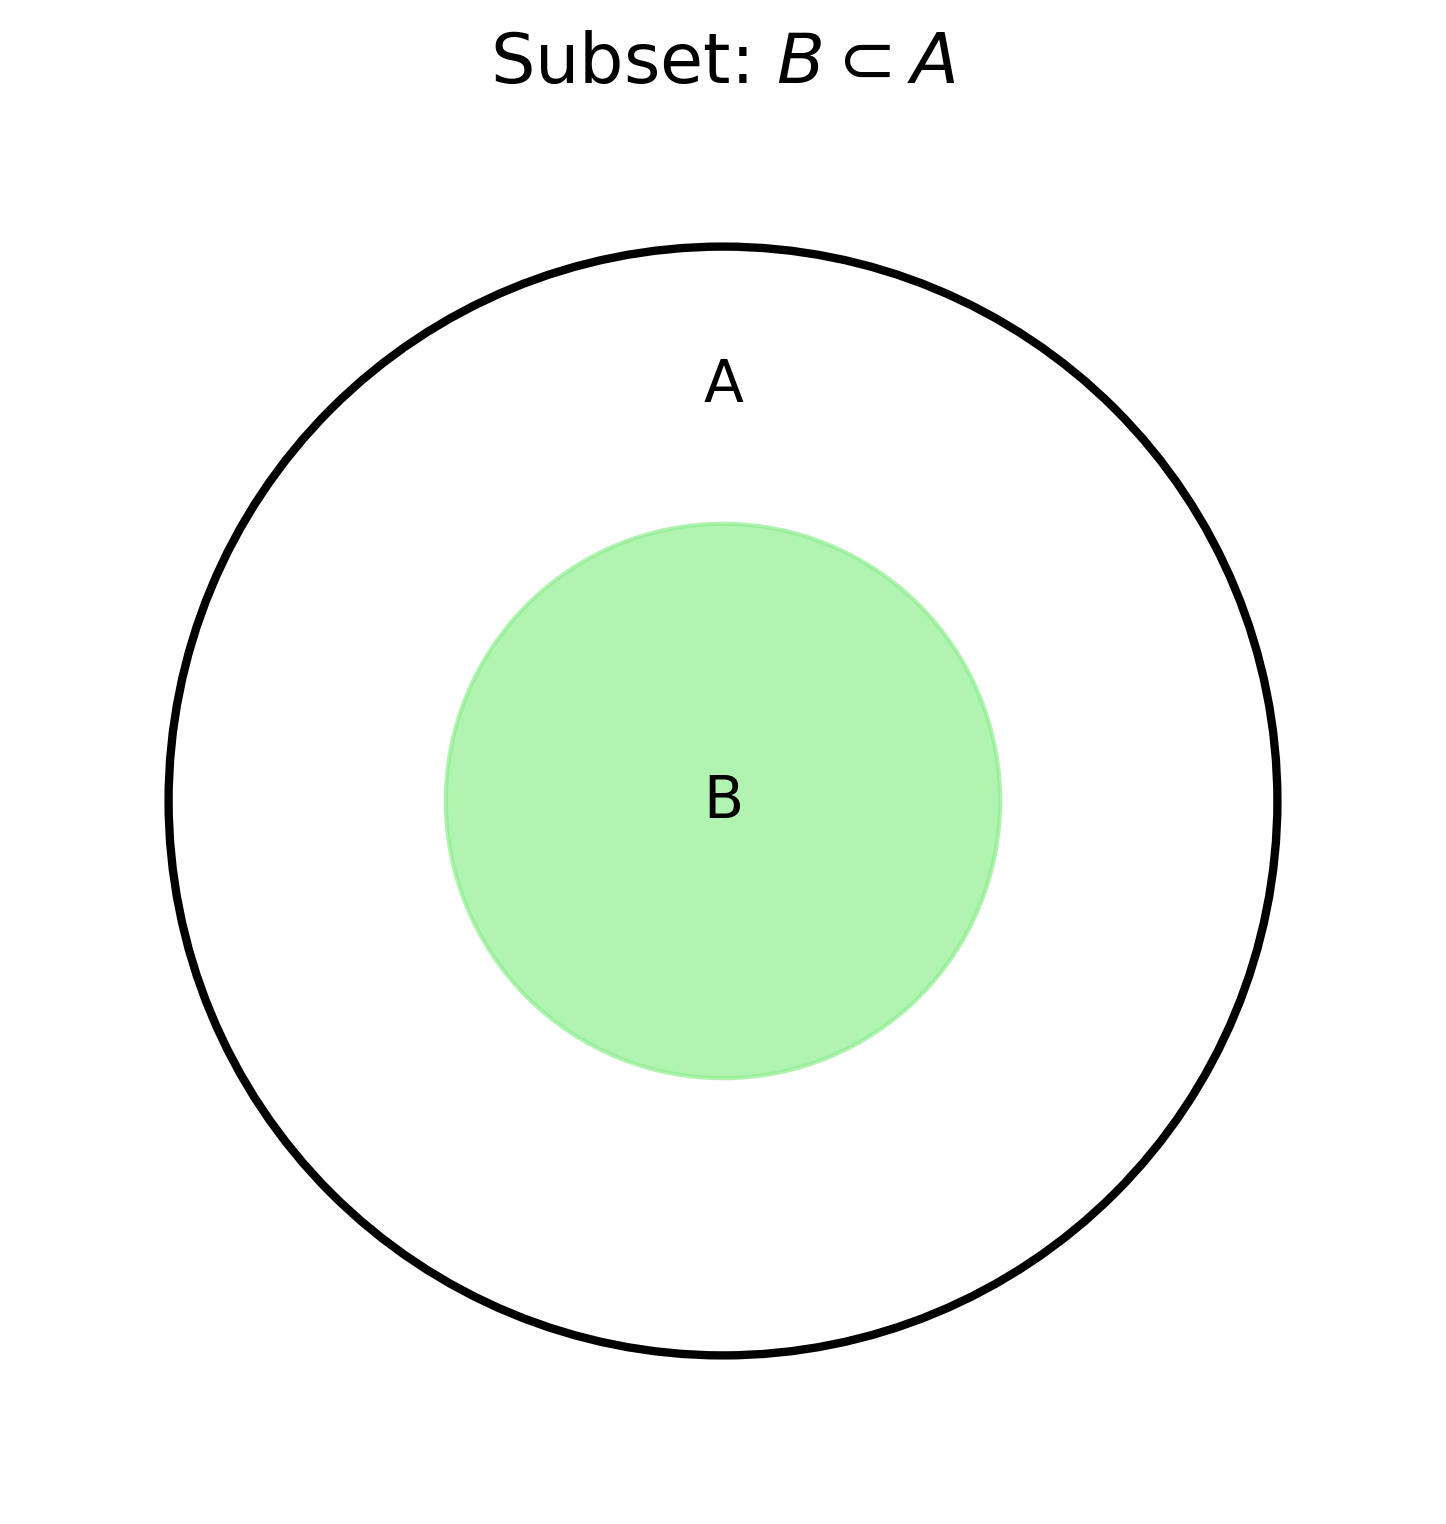
\includegraphics[width=\textwidth]{figures/set_operations/subset.png}
        \caption{Subset: $B \subset A$}
        \label{fig:subset}
    \end{subfigure}
    
    \vspace{0.5cm}
    
    \begin{subfigure}{0.48\textwidth}
        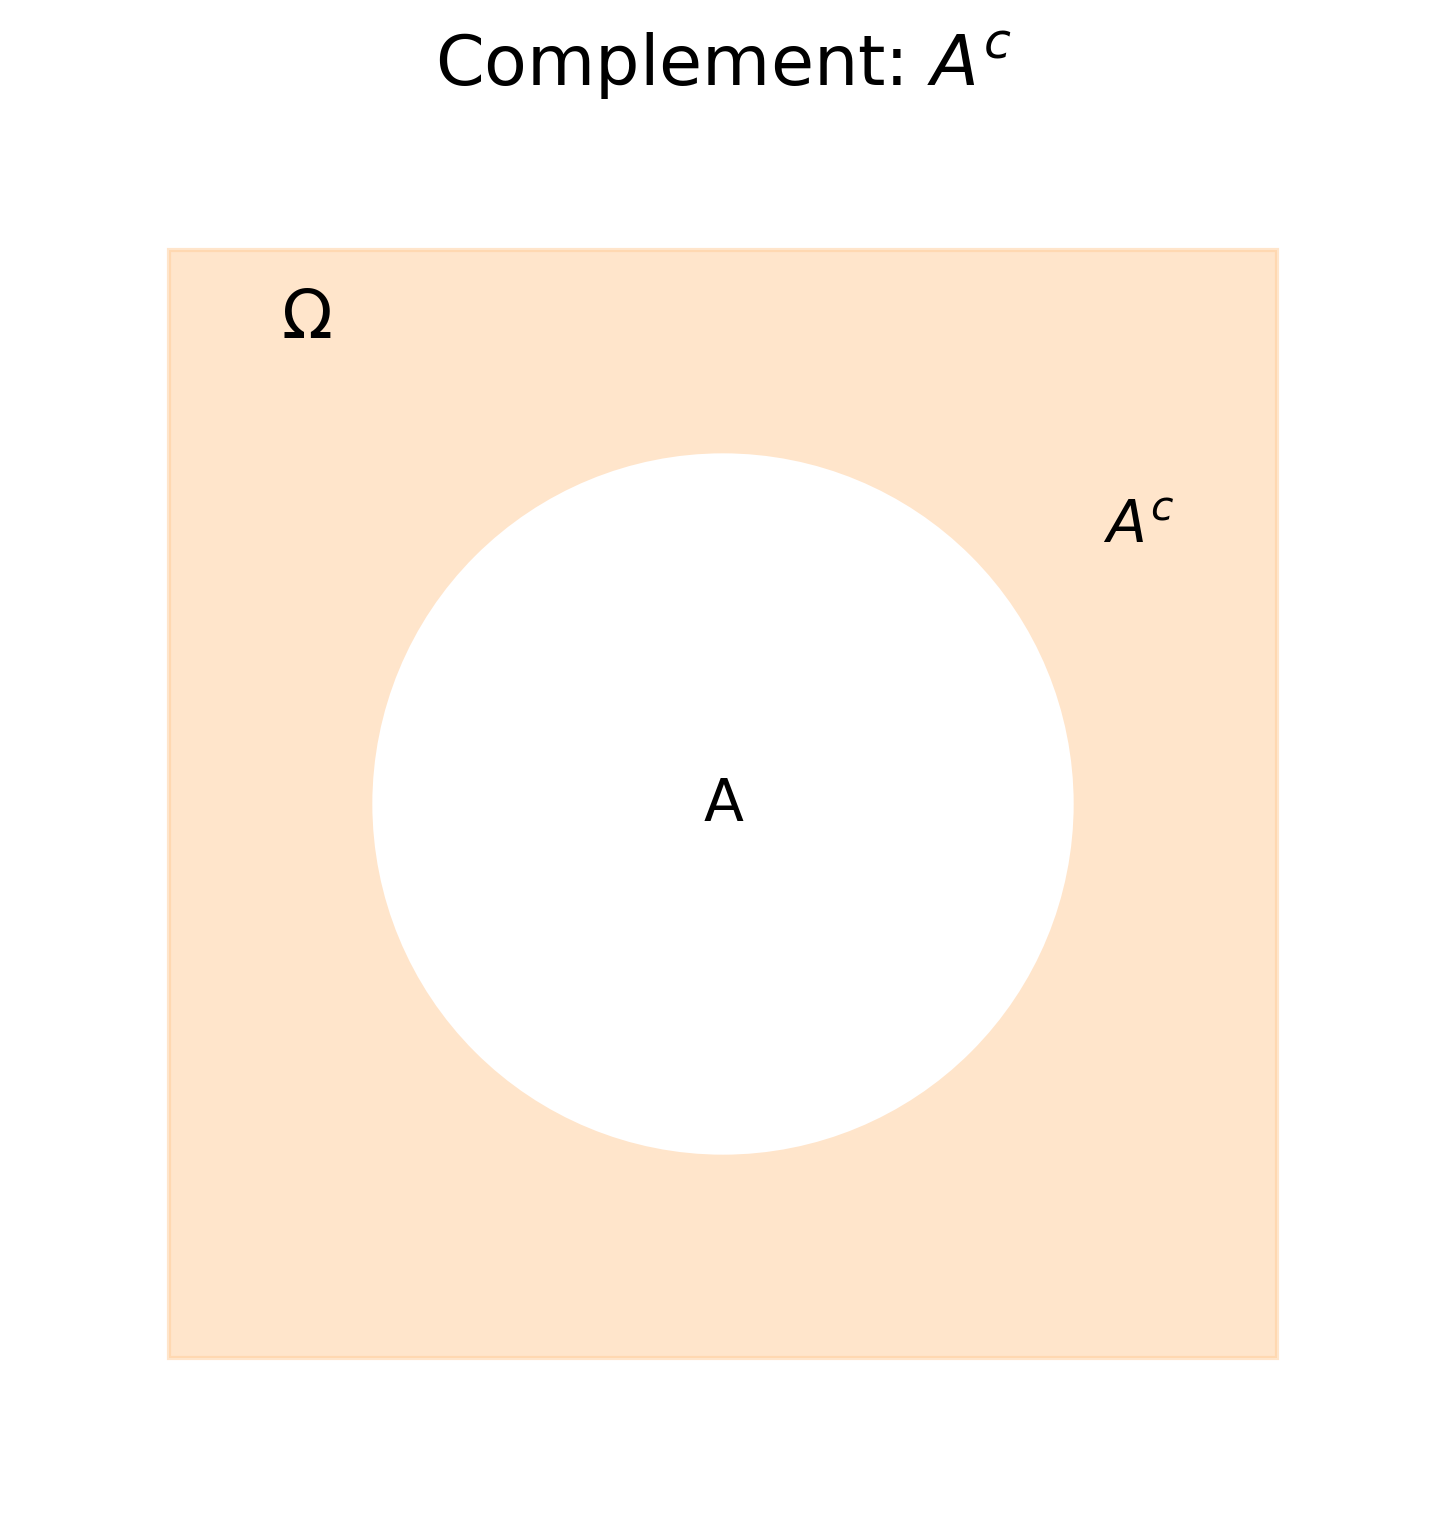
\includegraphics[width=\textwidth]{figures/set_operations/complement.png}
        \caption{Complement: $A^c$}
        \label{fig:complement}
    \end{subfigure}
    \hfill
    \begin{subfigure}{0.48\textwidth}
        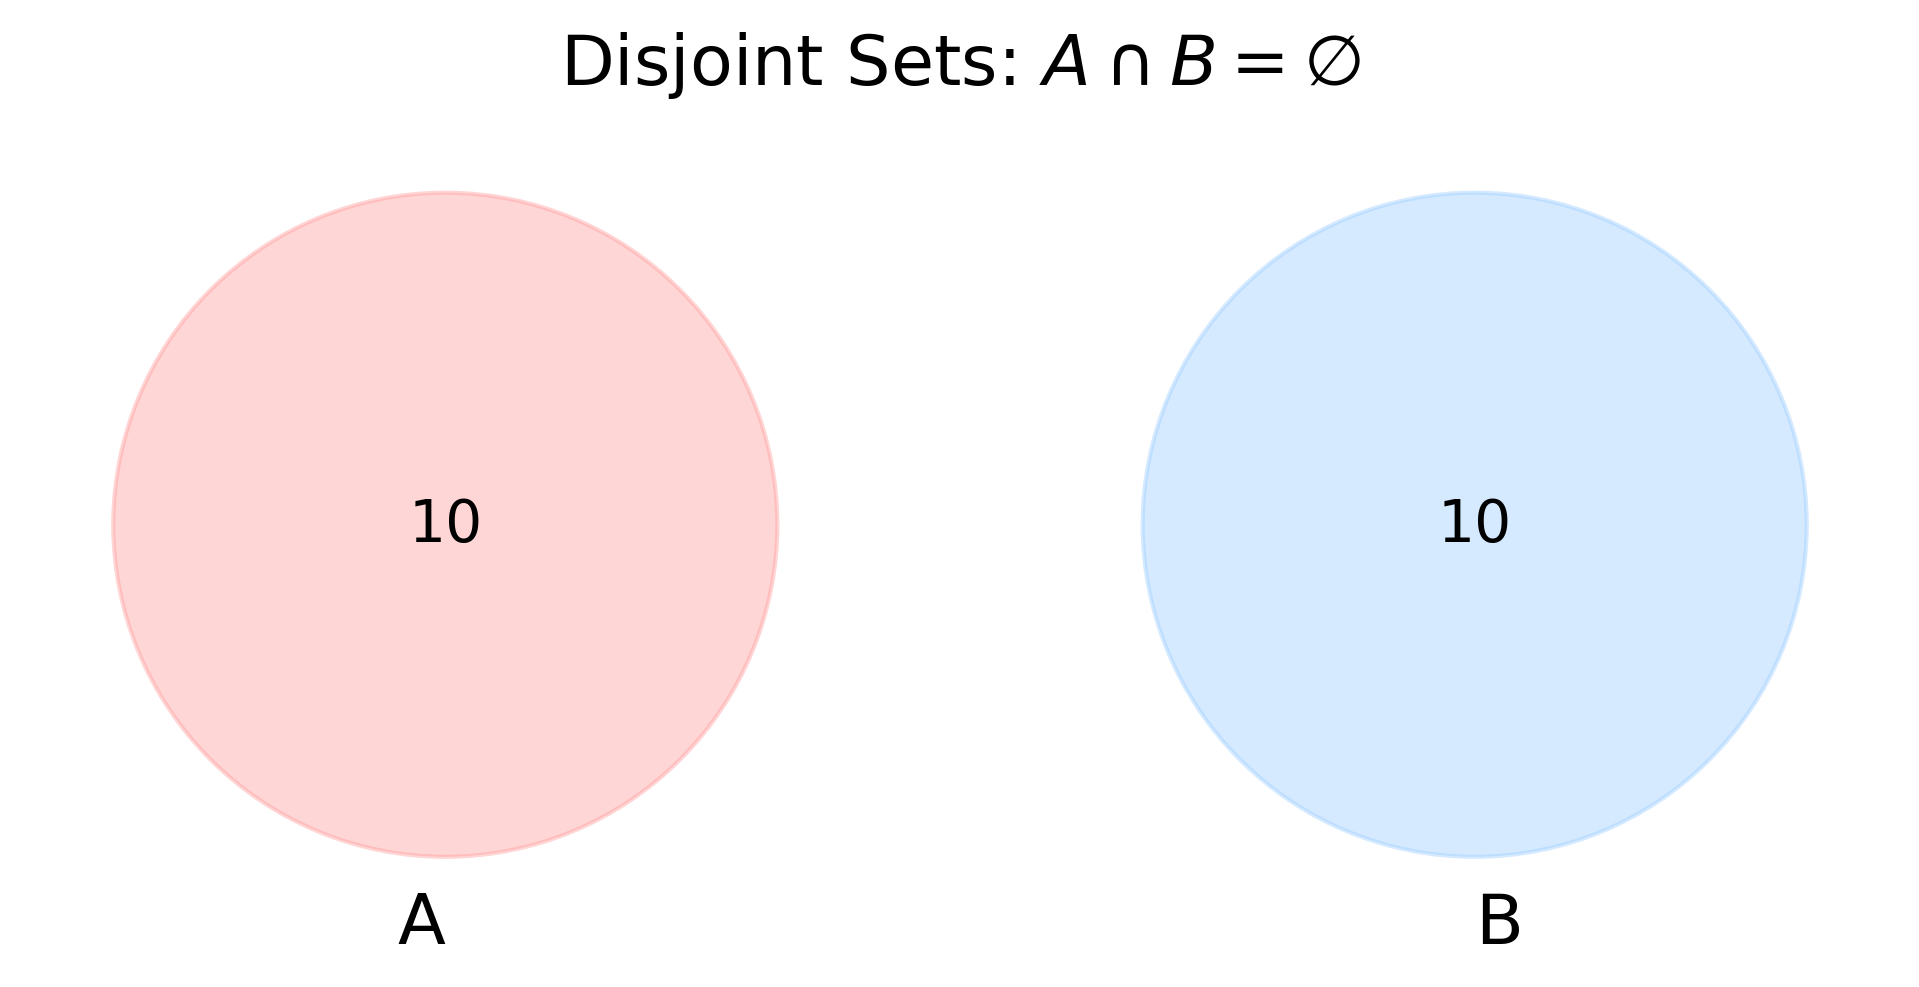
\includegraphics[width=\textwidth]{figures/set_operations/disjoint.png}
        \caption{Disjoint Sets: $A \cap B = \emptyset$}
        \label{fig:disjoint}
    \end{subfigure}
    
    \vspace{0.5cm}
    
    \begin{subfigure}{0.48\textwidth}
        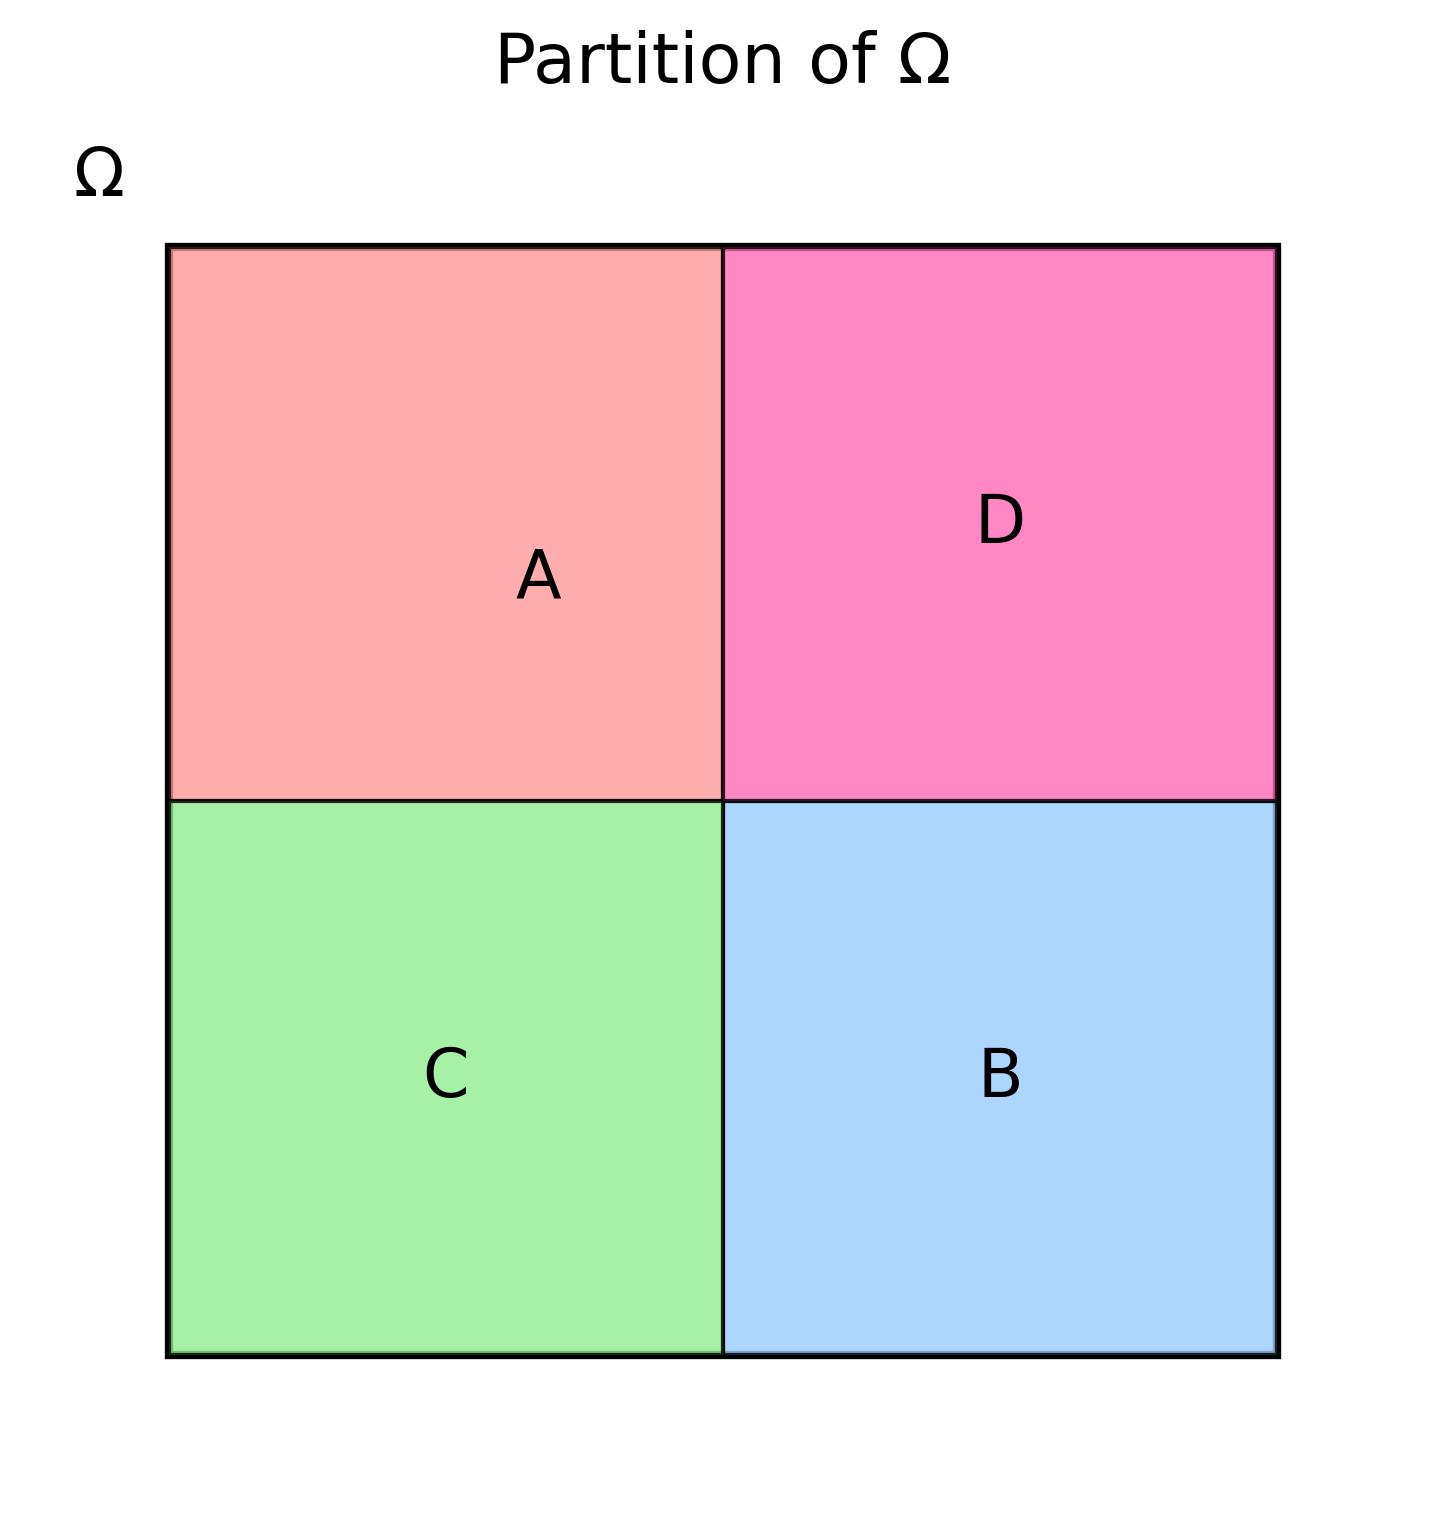
\includegraphics[width=\textwidth]{figures/set_operations/partition.png}
        \caption{Partition of $\Omega$}
        \label{fig:partition}
    \end{subfigure}
    \hfill
    \begin{subfigure}{0.48\textwidth}
        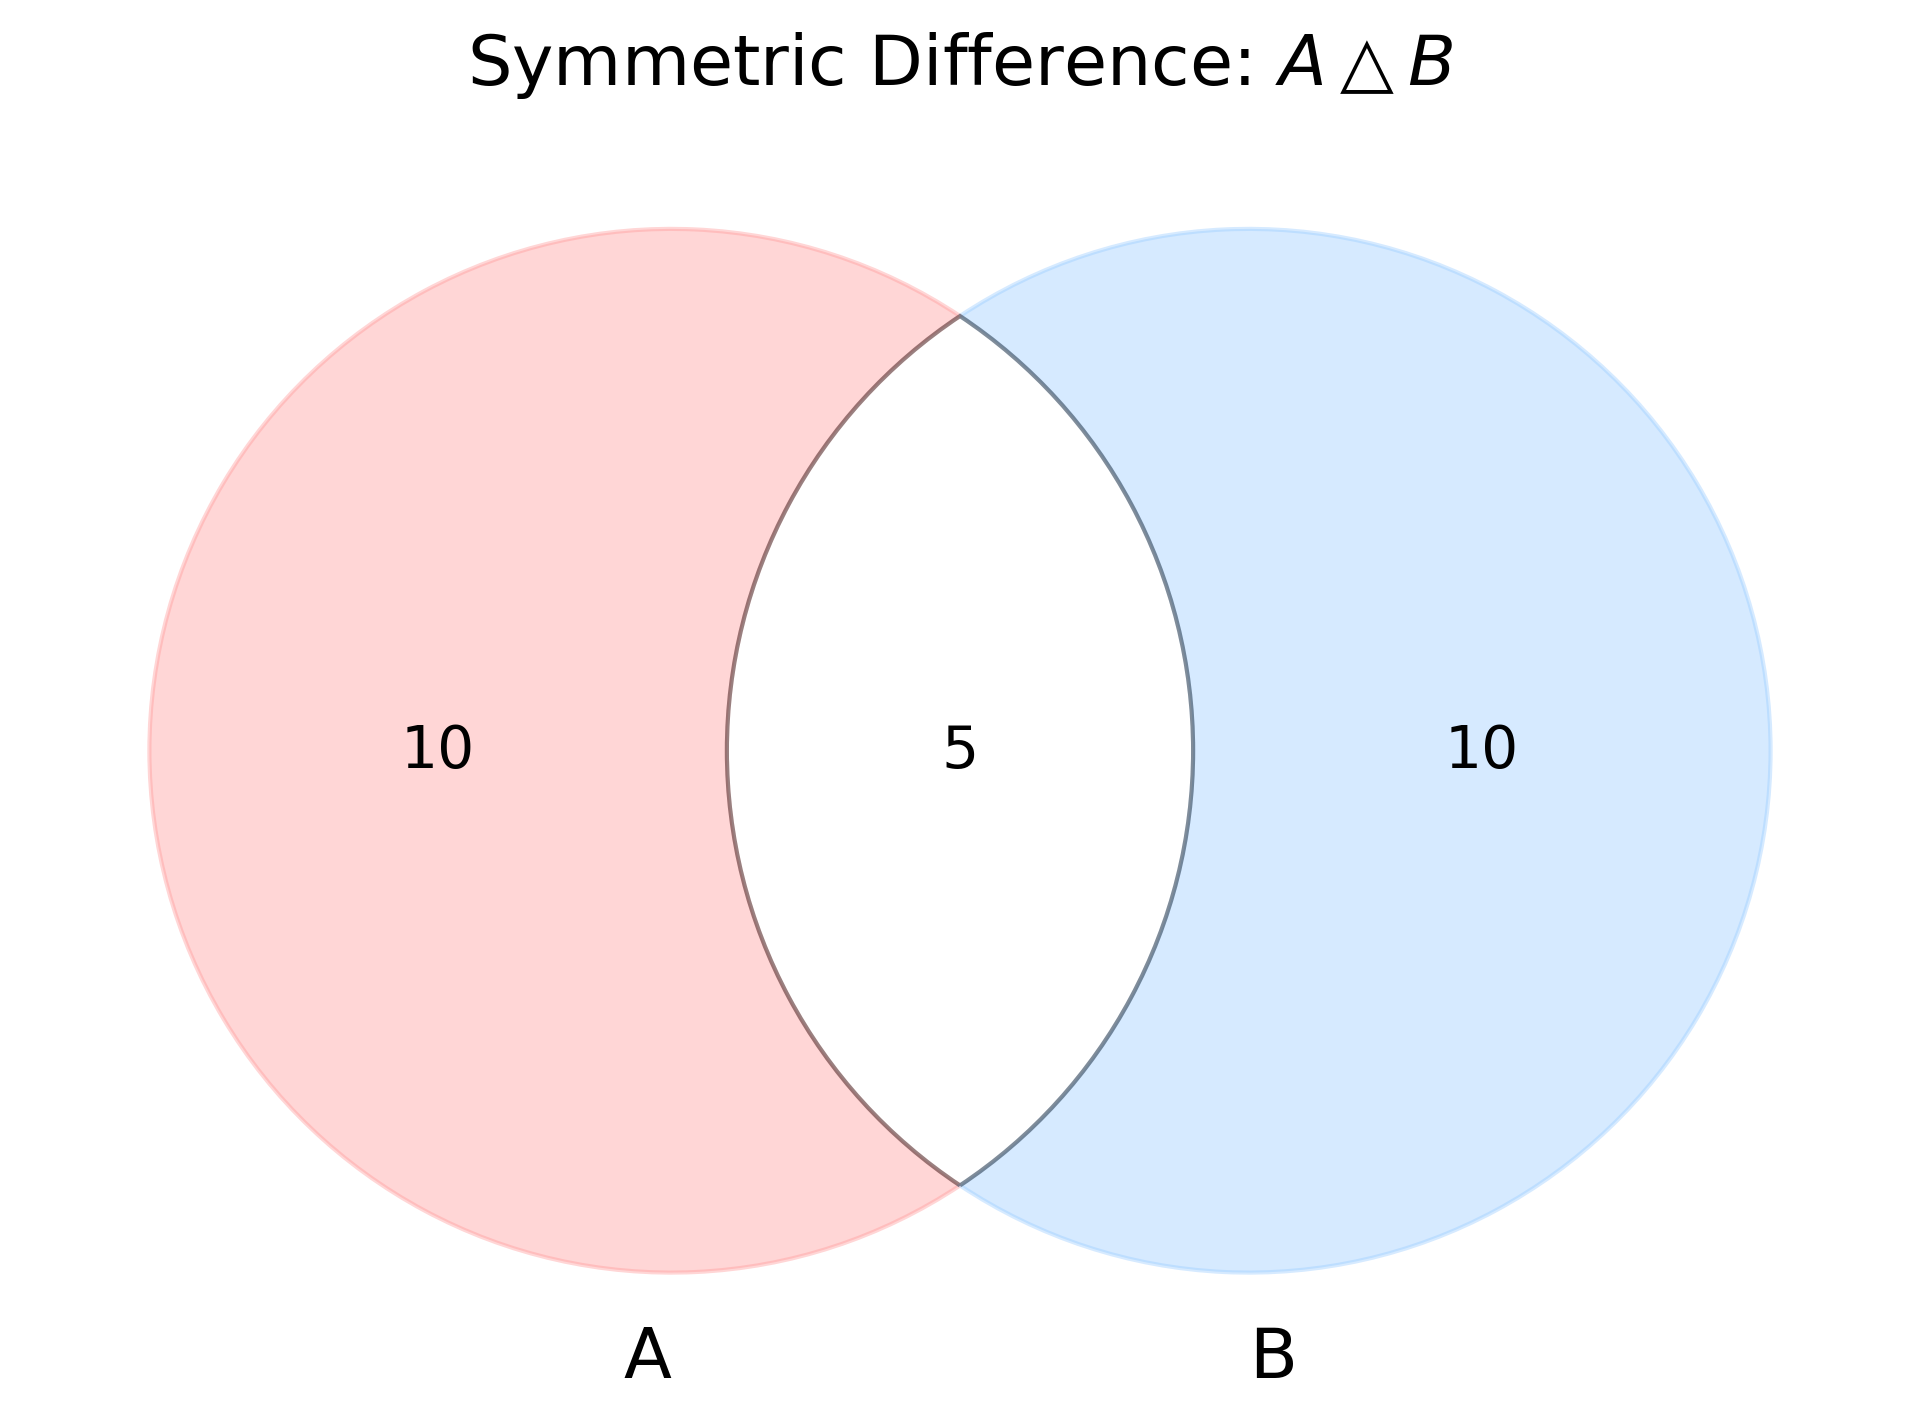
\includegraphics[width=\textwidth]{figures/set_operations/symmetric_difference.png}
        \caption{Symmetric Difference: $A \triangle B$}
        \label{fig:symmetric-difference}
    \end{subfigure}
    
    \caption{Visualizations of fundamental set operations generated with Matplotlib}
    \label{fig:set-operations}
\end{figure}

\subsection{Combined View of All Set Operations}

For a comprehensive overview of all set operations, you can use the combined figure:

\begin{figure}[h]
    \centering
    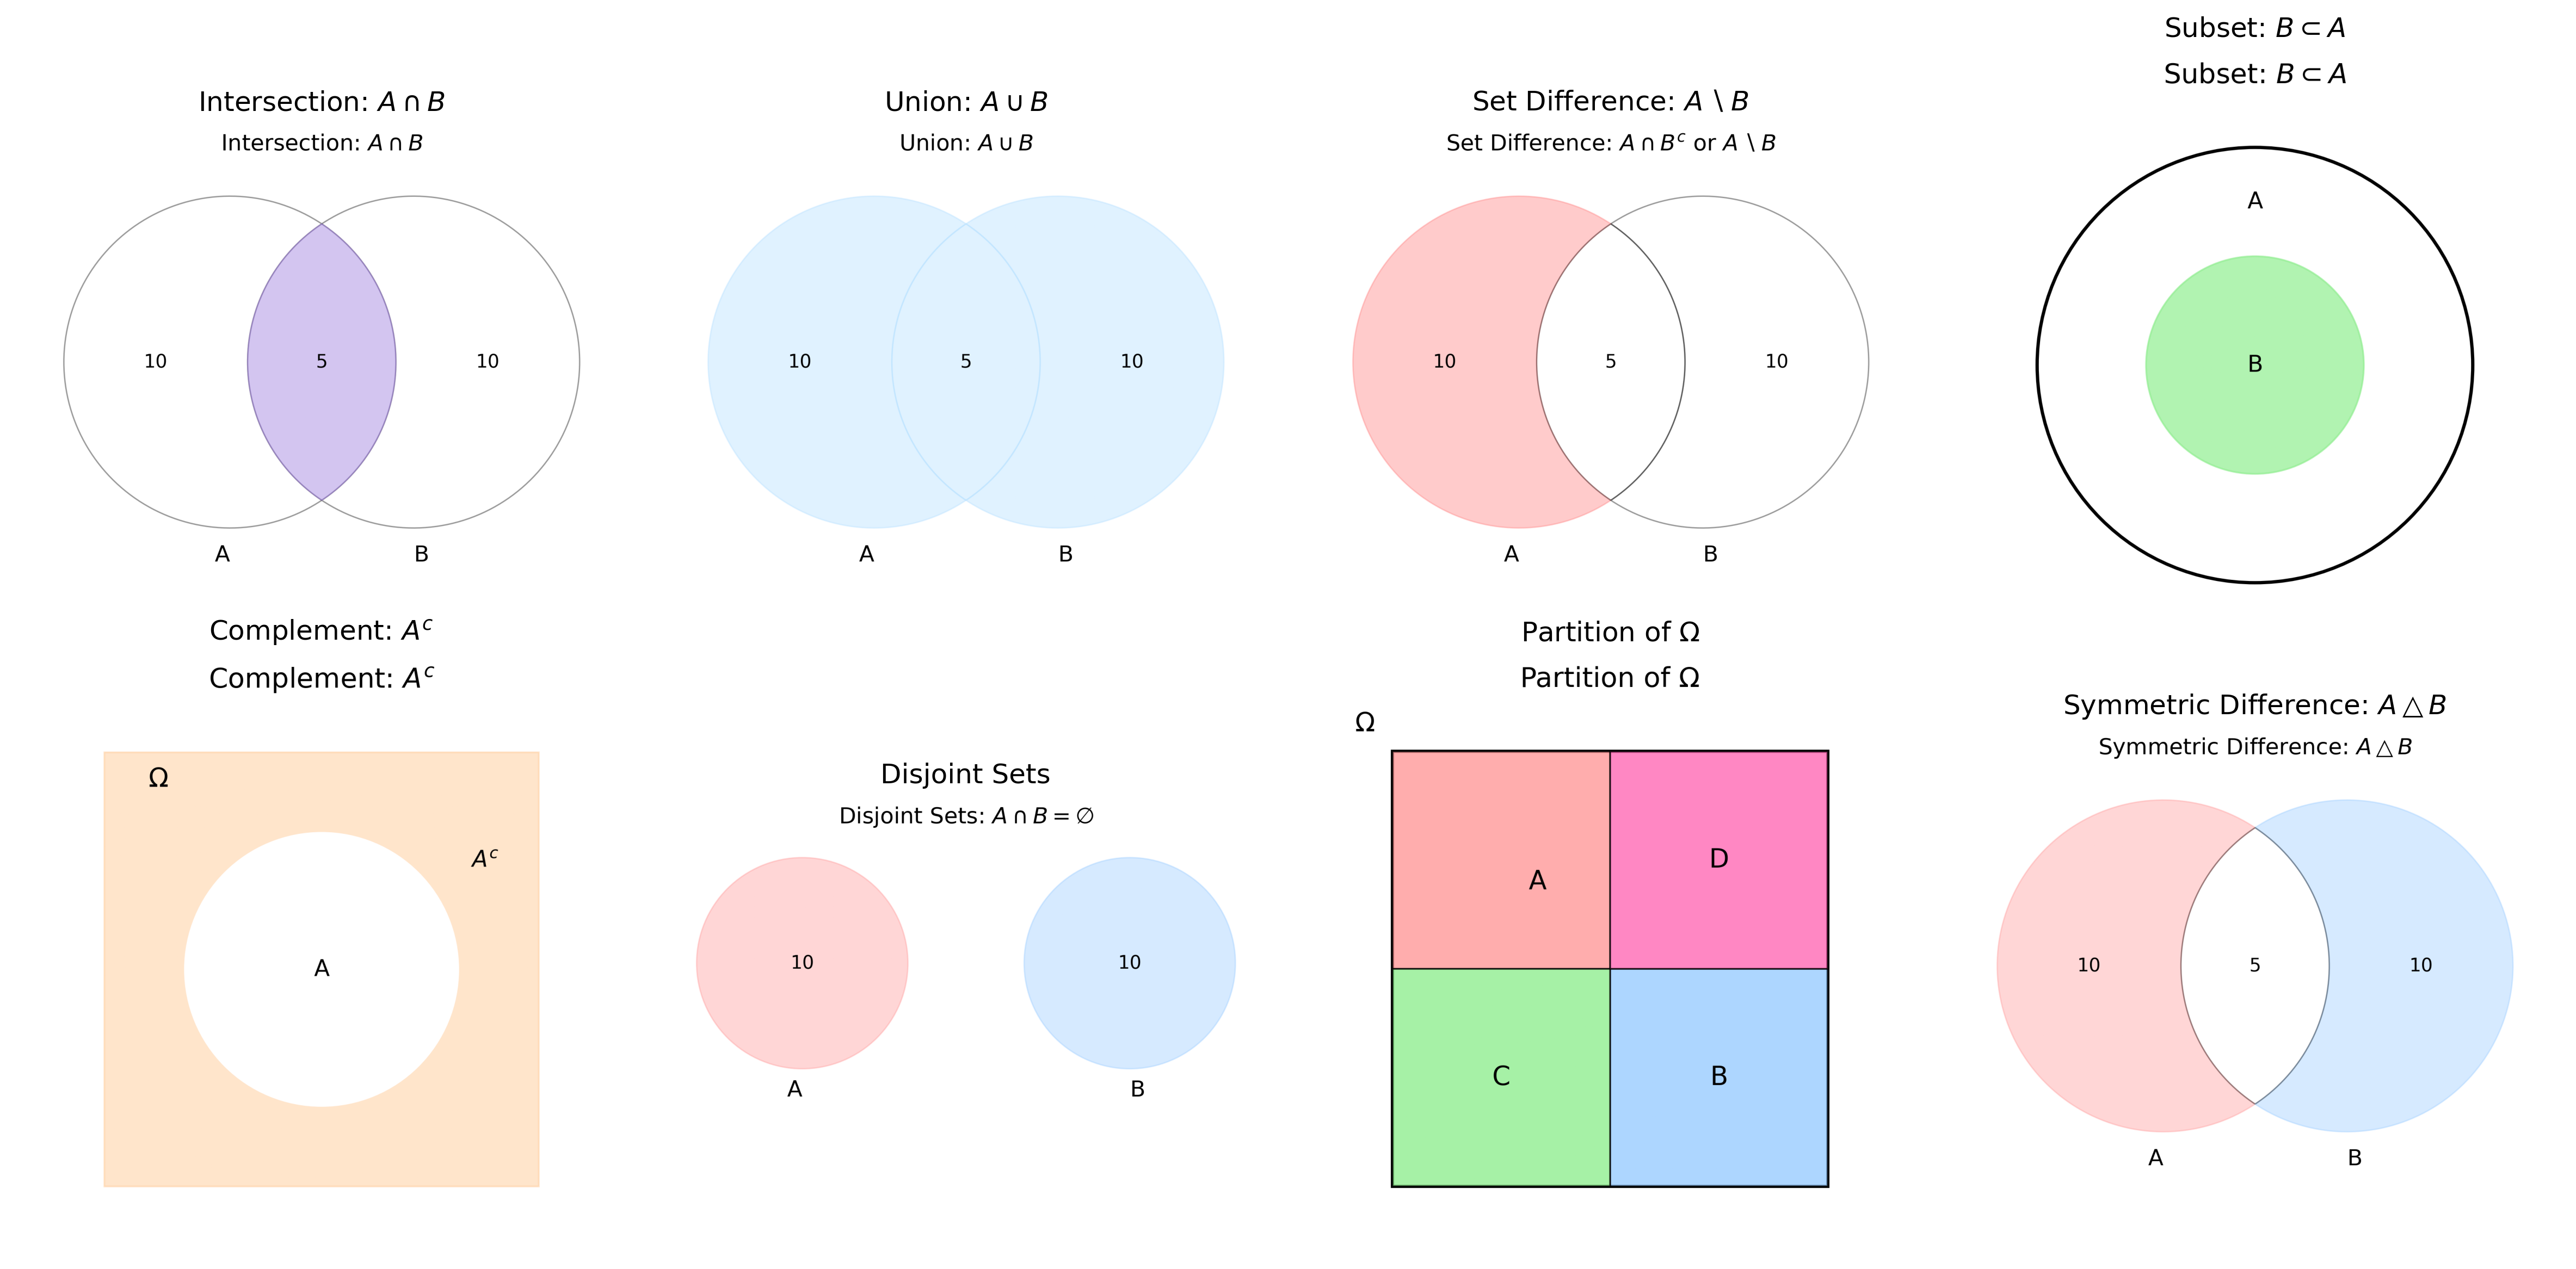
\includegraphics[width=\textwidth]{figures/set_operations/all_operations.png}
    \caption{Overview of fundamental set operations}
    \label{fig:all-set-operations}
\end{figure}

% Note: You'll need to adjust the relative path to the figures based on your document structure